\begin{figure}
    \centering
    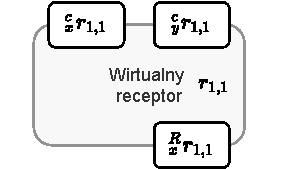
\includegraphics[width=0.75\columnwidth]{figures/ISR-vr-camera-model.pdf}
    \label{fig:model-vr-camera}
    \caption{Struktura ogólna wirtualnego receptora kamery RGB-D}
\end{figure}

\begin{figure}
    \centering
    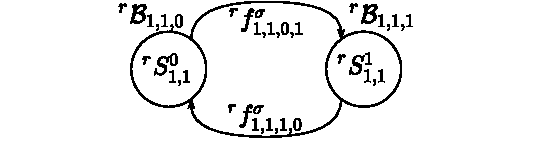
\includegraphics[width=\columnwidth]{figures/ISR-vr-camera-behaviours.pdf}
    \label{fig:zachowania-vr-camera}
    \caption{Automat zachowań wirtualnego receptora kamery RGB-D}
\end{figure}


Zachowania:
\begin{itemize}
    \item ${}^{r}\mathcal{B}_{1,1,0}$ - blocks,
    \item ${}^{r}\mathcal{B}_{1,1,1}$ - places,
\end{itemize}

Bufory komunikacyjne:
\begin{itemize}
    \item ${}^{c}_{x}r_{1,1} = \varphi \in \{b, p\}$ - tryb detekcji klocków/miejsc,
    \item ${}^{c}_{y}r_{1,1} = \Theta_{d}$ - pozycja wykrywanego klocka/miejsca,
    \item ${}^{R}_{x}r_{1,1} = \Lambda$ - chmura punktów z~kamery RGB-D.
\end{itemize}

Warunki początkowe:
\begin{itemize}
    \item ${}^{r}f^{\sigma}_{1,1,0,1} \triangleq \varphi = p$,
    \item ${}^{r}f^{\sigma}_{1,1,1,0} \triangleq \varphi = b$
\end{itemize}

Warunki końcowe:
\begin{itemize}
    \item ${}^{r}f^{\tau}_{1,1,0} \triangleq \varphi \neq b$,
    \item ${}^{r}f^{\tau}_{1,1,1} \triangleq \varphi \neq p$
\end{itemize}

Wymagane funkcje pomocnicze:
\begin{itemize}
    \item $detect(\Lambda)$ - wykryj żółty sześciany
    \item $getTF(c)$ - zwróć pozycję podanego sześcianu,
    
    \item $find(\Lambda)$ - wykryj możliwe położenia do odstawienia,
    \item $getFinal(s)$ - zwróć pozycję docelowego położenia do odstawienia sześcianu.
\end{itemize}

Funkcje przejścia w postaci matematycznej:
\begin{itemize}
    \item \textbf{blocks} \begin{itemize}
        \item ${}^{r_{1,1}, c_{1,1}}f_{1,1,0} \triangleq {}^{c}_{y}e_{1,1} = getTF(detect({}^{R}_{y}r_{1,1}))$
    \end{itemize} 
    \item \textbf{places} \begin{itemize}
        \item ${}^{r_{1,1}, c_{1,1}}f_{1,1,1} \triangleq {}^{c}_{y}e_{1,1} = getFinal(find({}^{R}_{y}r_{1,1}))$
    \end{itemize}
\end{itemize}

\begin{figure}
    \centering
    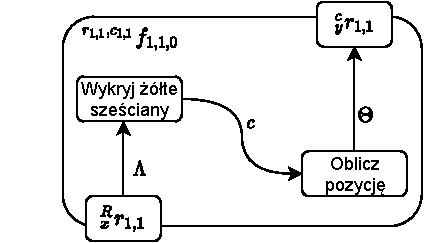
\includegraphics[width=\columnwidth]{figures/ISR-vr-camera-fp-blocks.pdf}
    \label{fig:vr-camera-fp-blocks}
    \caption{Zdekomponowana funkcja przejścia zachowania \textbf{blocks} w~postaci DFD}
\end{figure}

\begin{figure}
    \centering
    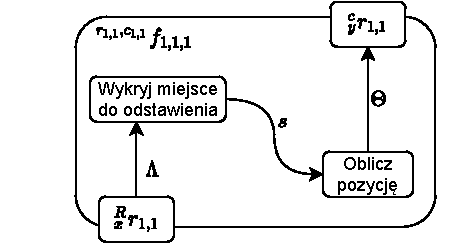
\includegraphics[width=\columnwidth]{figures/ISR-vr-camera-fp-places.pdf}
    \label{fig:vr-camera-fp-places}
    \caption{Zdekomponowana funkcja przejścia zachowania \textbf{places} w~postaci DFD}
\end{figure}